
\section{Result: DMPcreator}
The result of our implementation efforts is the user friendly webinterface \texttt{DMPcreator}. It enables scientists to create a data management plan based on the .tsv file produced by \texttt{QWizard}. The tool is structured into five slides. A progress bar on top of every slide gives an excellent overview of the current advances. Furthermore, the user can navigate through the slides by clicking at the buttons at the bottom on the right (present in every slide). Moreover, every slide contains a detailed description about what, where and why the user has to fill in here. Note, that every field in every slide will be parsed in the end and the information is stored in a human readable PDF file.\par
The first slide, the \textit{General Information Slide}~(figure \ref{GeneralInformationSlide}), provides fields letting the user enter general information about his project, for example the project name, the person in charge of the project and contact data. Furthermore, the user can upload his .tsv file created by \texttt{Q-Wizard}. From this uploaded data experiment details like species, experiment types, number of experiment per experiment type, and so forth are extracted for later usage (slide \textit{Storage \& Backup} (figure \ref{StorageBackupSlide}) needs this information in order to calculate required storage correctly). \par
One important topic that needs to be covered when creating a data management plan is \textit{Roles \& Responsibilities}~(figure \ref{RolesResponsibilitiesSlide}) of every project member. This second slide allows the user to assign roles to persons. The chosen values are added to a responsibilities list later being parsed by the PDF creator. \par Having specified who is responsible for which data, the user still has to decide, how the data is stored. Here steps the third slide \textit{ContentManagement} (figure \ref{ContentManagementSlide}) in. The user can assign file types to an associated description building a content. PDF creator parsed these user created contents, too. \par
How to store data efficiently is one key component in a data management plan. In the slide \textit{Storage \& Backup} (figure \ref{StorageBackupSlide}) the user is able to fill in the storage location, the RAID backup solution, the archive solution and how much data (in GB) one experiment will produce approximately. Changing the needed disk space for an experiment results in an update of the displayed total required space. So the user gets an immediate feedback when filling in necessary fields. \par
The last slide covers the topic of \textit{Dissemination} (figure \ref{Dissemination}) of data. This mask provides fields for the user to generate dissemination methods. Furthermore, by clicking on the 'Generate Report' button, the PDF creator produces the PDF. Another button ('Download Report') then allows the user to download the created report.
\begin{landscape}
	\begin{figure}[]
		\centering
		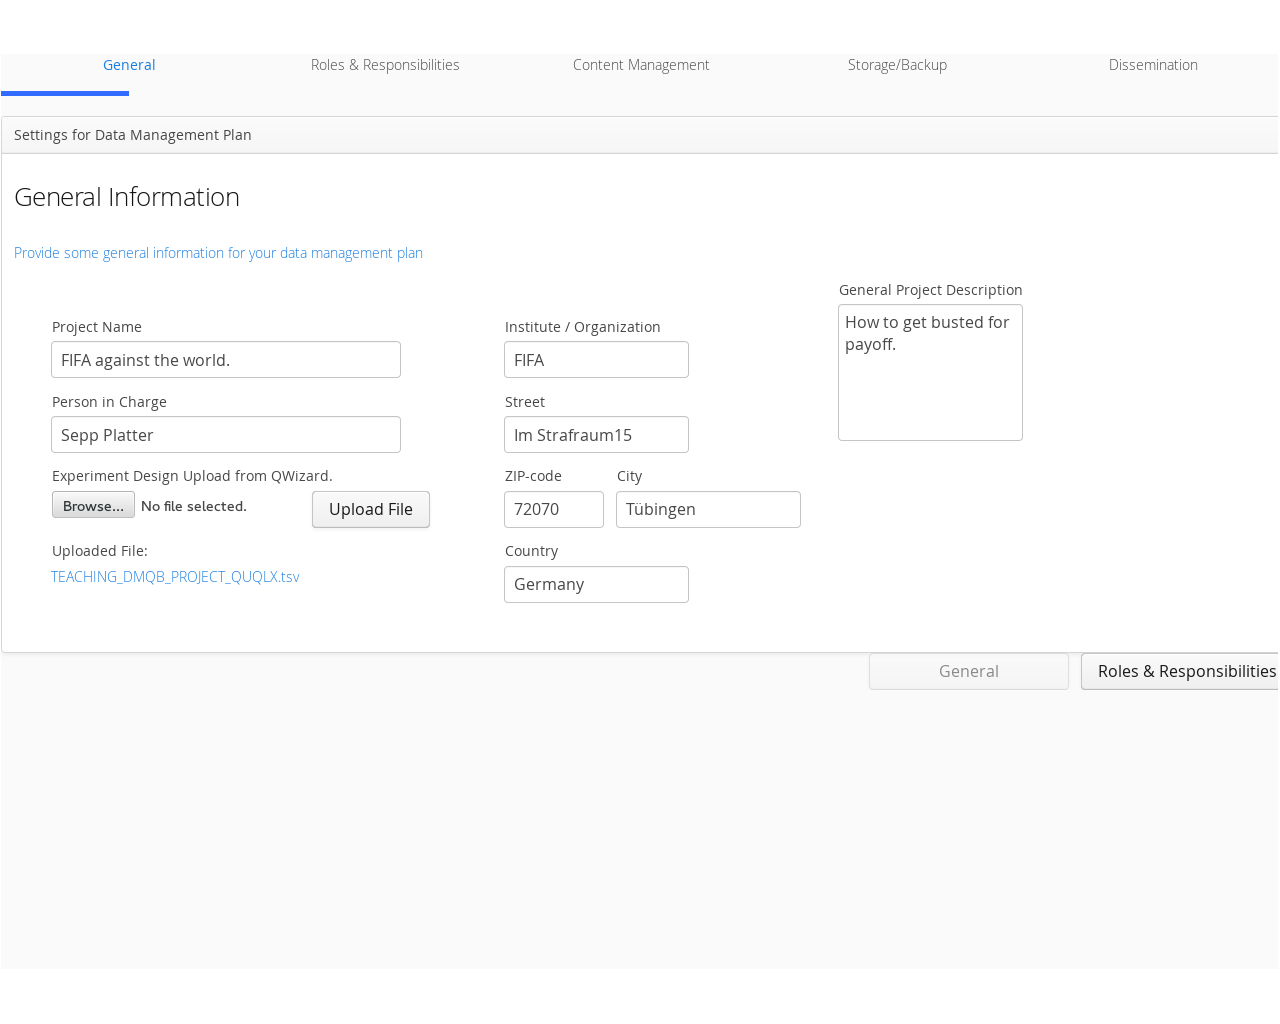
\includegraphics[width=1.2\textwidth]{pictures/GeneralInformation.png}
		\caption{\textit{General Information} Slide of \texttt{DMPcreator}. The progress bar is placed on the top. Fields that are fillable by the user can be seen below. Note, a special upload field for the .tsv file from \texttt{Q-Wizard} is visible on the left bottom.}
		\label{GeneralInformationSlide}
	\end{figure}

\begin{figure}[]
	\centering
	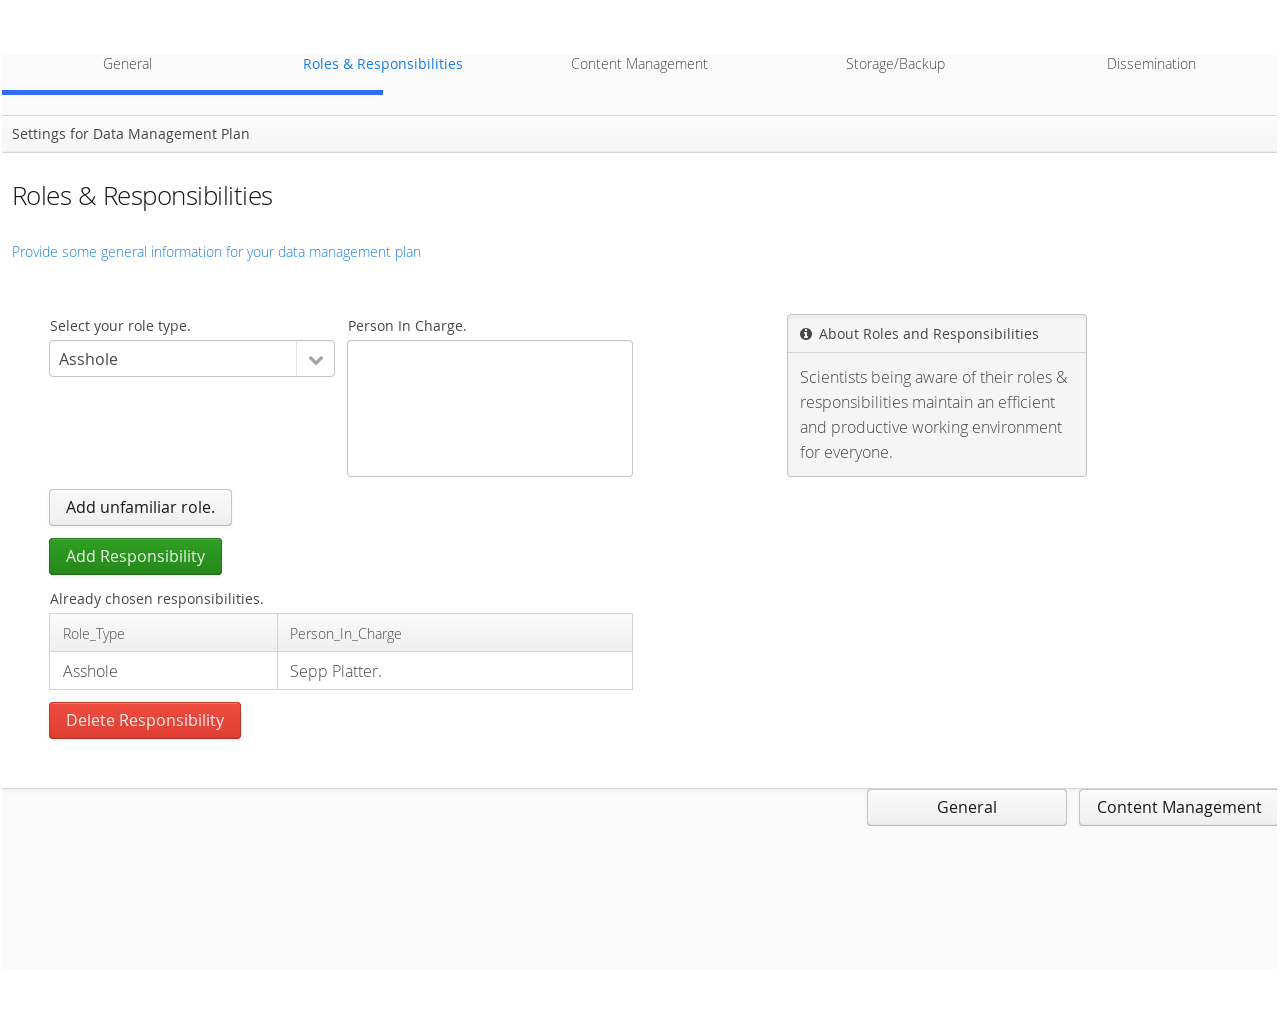
\includegraphics[width=1.2\textwidth]{pictures/RolesResponsibilities.png}
	\caption{\textit{Roles \& Responsibilities} Slide of \texttt{DMPcreator}. The progress bar is placed on the top. Fields that are fillable by the user can be seen below.}
	\label{RolesResponsibilitiesSlide}
\end{figure}

\begin{figure}[]
	\centering
	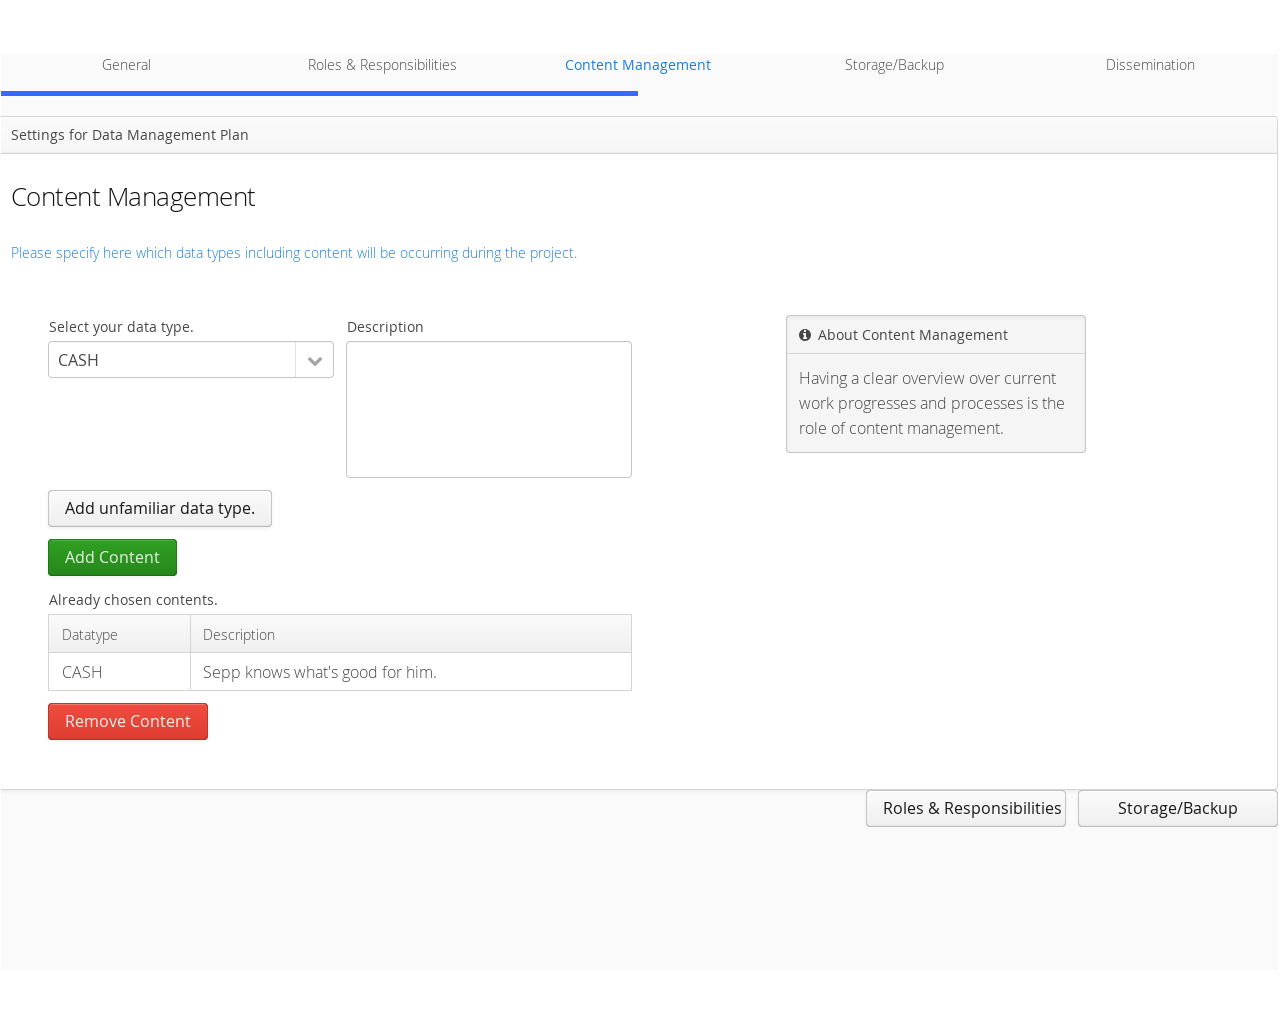
\includegraphics[width=1.2\textwidth]{pictures/ContentManagement.png}
	\caption{\textit{Content Management} Slide of \texttt{DMPcreator}. The progress bar is placed on the top. Fields that are fillable by the user can be seen below.}
	\label{ContentManagementSlide}
\end{figure}

\begin{figure}[]
	\centering
	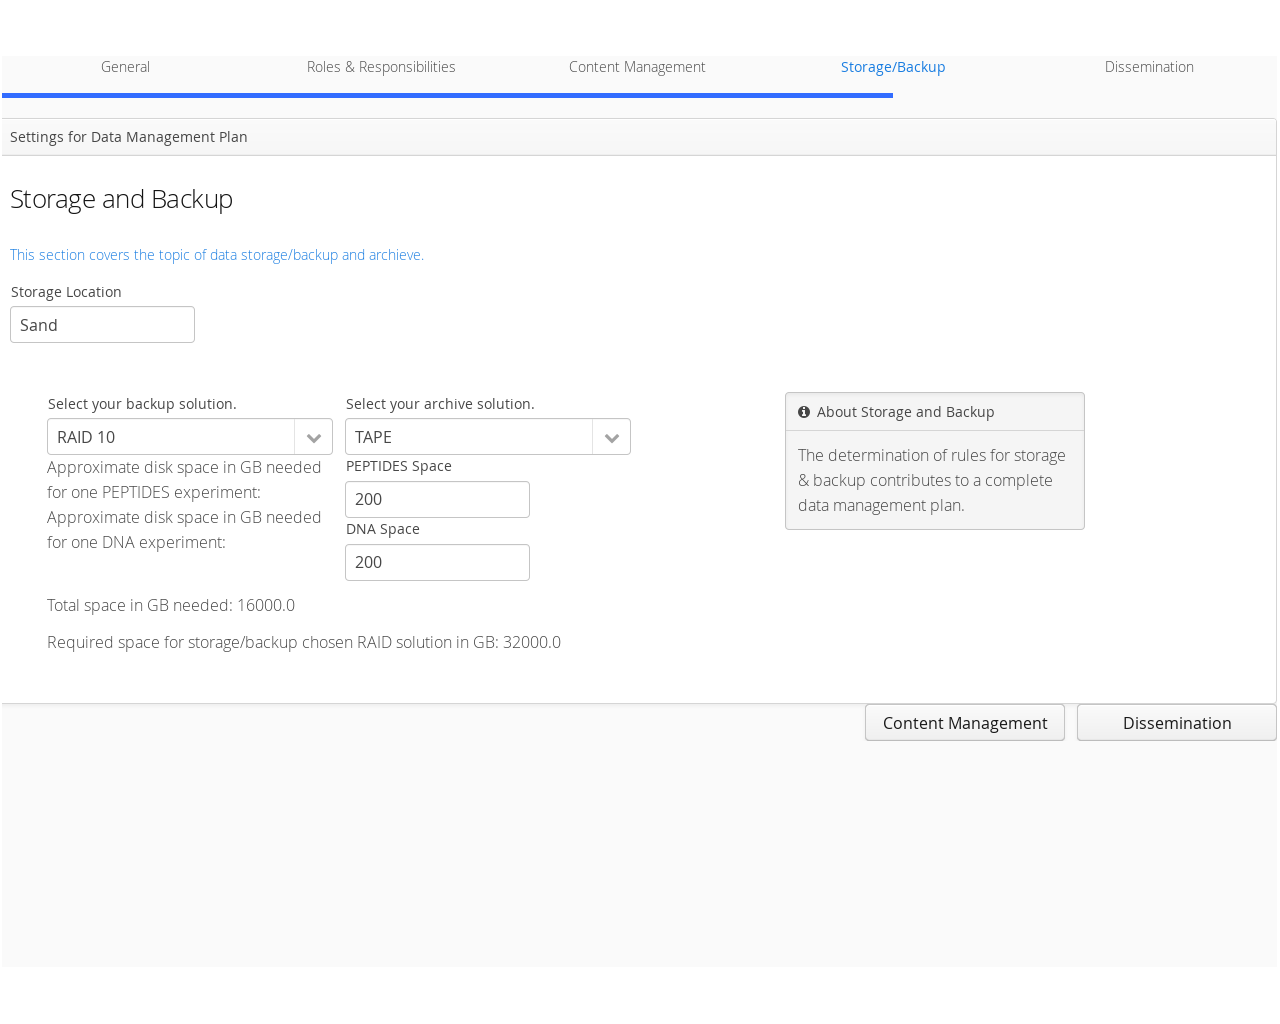
\includegraphics[width=1.2\textwidth]{pictures/StorageBackup.png}
	\caption{\textit{Storage \& Backup} Slide of \texttt{DMPcreator}. The progress bar is placed on the top. Fields that are fillable by the user can be seen below.}
		\label{StorageBackupSlide}
\end{figure}

\begin{figure}[]
	\centering
	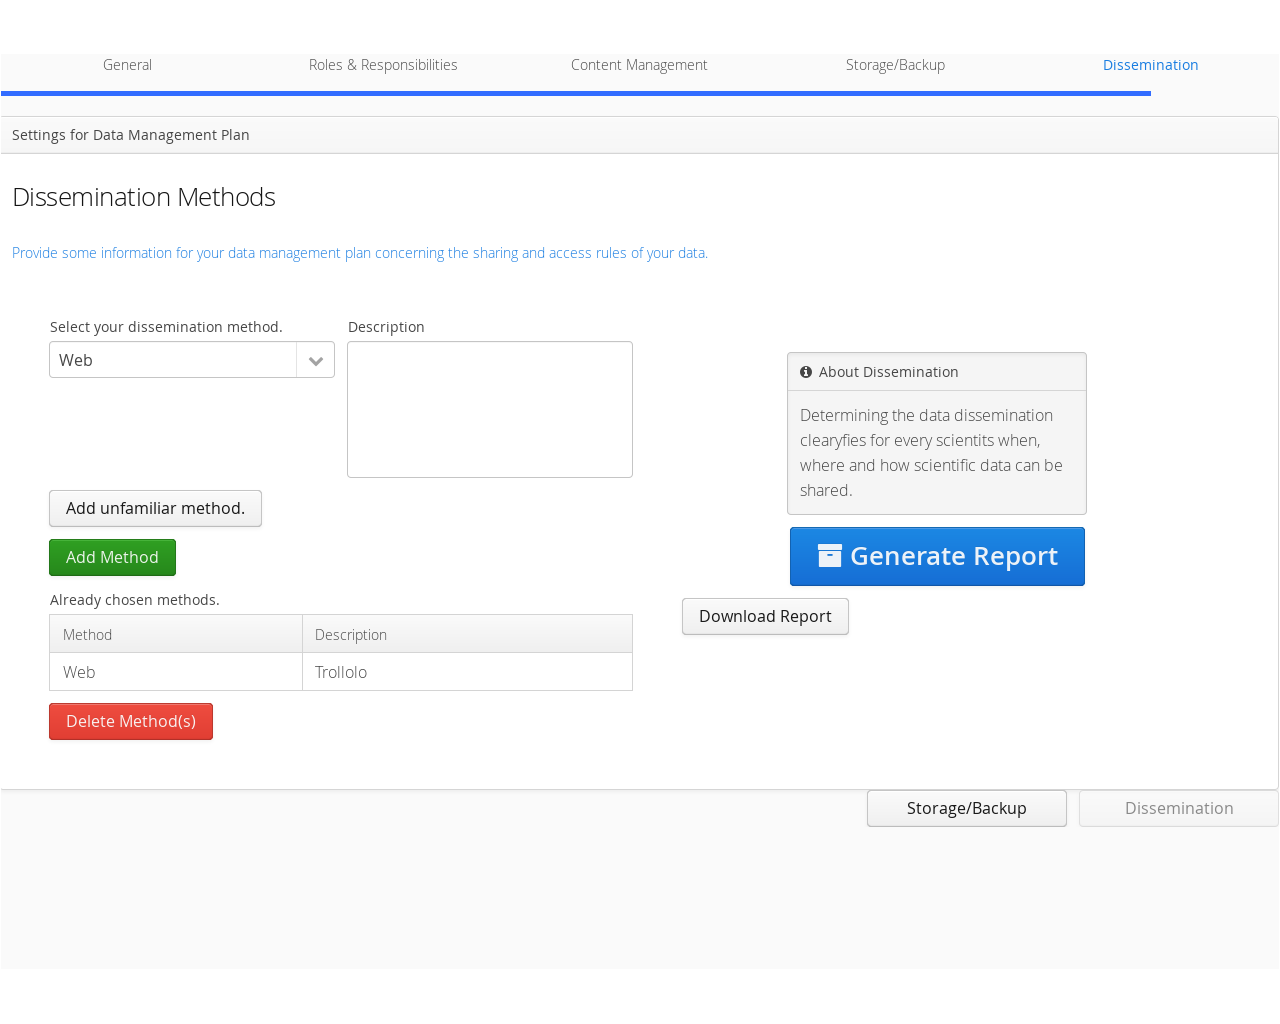
\includegraphics[width=1.2\textwidth]{pictures/Dissemination.png}
	\caption{\textit{Dissemination} Slide of \texttt{DMPcreator}. The progress bar is placed on the top. Fields that are fillable by the user can be seen below.}
	\label{Dissemination}
\end{figure}
\end{landscape}